\documentclass[a4paper,10pt]{article}
\usepackage[utf8]{inputenc}
\usepackage[pdftex]{graphicx}
\usepackage{caption}
\usepackage{subcaption}
\usepackage{verbatim}

%opening
\title{Filtro Digital IIR utilizando aproximação Elíptica}
\author{Danilo Souza, Hugo Santos, Welton Araújo}

\begin{document}

\maketitle

\section{Introdução}
%Existe uma necessidade muito grande em processamento de sinais em tratar sinais de entrada em uma determinada banda de frequência. Isto só é possível por meio de uma função de transferência com uma razão de polinômios para gerar filtros com resposta ao impulso de duração infinita(IIR).

%Filtros IIR têm uma melhor aplicação prática por conta de precisar de menos multiplicações para realizar uma aproximação. Diferentemente de filtros com resposta ao impulso finitas(FIR), pois possuem mais dificuldade na atuação em processamento de sinais em tempo real.

%O método de aproximação adotado neste trabalho, o elíptico, tem sua origem no domínio do tempo contínuo. Por conseguinte, é necessária uma transformação para o tempo discreto, através da transformação bilinear.

Devido à grande dificuldade para se trabalhar com sinais reais, em função da grande  presença de rúido existente universo analógio, a utilização de filtros é de fundamental fundamental importância para processamento digital de sinais, atuando a na eliminção de ruído indesejado, e preservação do sinal de interesse. Esta operação é feita no domínio da frequência, onde o filtro possui uma resposta em frequência composta por magnitude e fase, uma vez que a saída de um Sistema Linear e Invariante no tempo é dada pela convolução da entrada com a resposta ao impulso do sistema, que, no domínio da frequência, corresponde à multiplicação da Resposta em Frequência pela transformada de Fourier do sinal de entrada. A fase da Resposta em Frequência indica a defasagem do sinal com relação ao sinal de entrada do sistema de filtragem e a resposta em magnitude representa as bandas de passagem, de corte e de transição, sendo esta última um ponto chave no projeto de filtros, uma vez que, dependo da aplicação, pode ser crucial ter uma banda de transição pequena, enquanto que em outros casos não é necessária uma grande rigidez para essa faixa de frequências do espectro.
 
Os filtros digitais são divididos em duas categorias, FIR (Resposta ao Impulso Infinita) e IIR (Resposta ao Impulso Infinita), sendo esta última apenas o mapeamento de filtros analógicos amplamente conhecidos e estudados, como Filtro de Chebyshev, Butterworth e Elíptico (Cauer), para o universo digital. 
Este trabalho tem por objetivo mostrar um implementação do filtro Elípitco, usando o MatLab, tomando como referência dois filtros, um passa-baixa e outro rejeita-faixa, descritos abaixo:   


\subsection{Filtro I}
Trata-se de um filtro passa-baixa. Suas especificações estão inseridas na Tabela \ref{tab:tabfiltro1}. Onde \(A_p\) e \(A_r\) são a atenuação máxima e mínima nas frequências de passagem e rejeição, respectivamente. E \(\Omega_p\), \(\Omega_r\) e \(\Omega_s\) são as frequências de máxima de passagem, mínima de rejeição e de amostragem, respectivamente.

\begin{table}
\centering
\begin{tabular}{|l|l|}

\(A_p\) 	& 1 dB		\\
\(A_r\) 	& 40 dB		\\
\(\Omega_p\) 	& 1000 Hz	\\
\(\Omega_r\) 	& 1290 Hz	\\
\(\Omega_s\) 	& 3000 Hz	\\

\end{tabular}
\caption{Propriedades do filtro I}
\label{tab:tabfiltro1}
\end{table}

\subsection{Filtro II}
Trata-se de um filtro rejeita-faixa. Suas especificações estão inseridas na Tabela \ref{tab:tabfiltro2}. Onde \(A_{p1}\) e \(A_{r1}\) são a atenuação máxima e mínima nas frequências de passagem e rejeição, respectivamente. \(\Omega_{p1}\) e \(\Omega_{r1}\) são as frequências  máxima de passagem e mínima de rejeição, respectivamente, da faixa inicial. \(\Omega_{p2}\), \(\Omega_{r2}\) são as frequências mínima de passagem, máxima de rejeição, respectivamente, da faixa final.
A frequ\^encia de amostragem \'e representada por \(\Omega_s\).

\begin{table}[ht]
\centering
\begin{tabular}{|l|l|}

\(A_p\) 	& 0,5 dB	\\
\(A_r\) 	& 60 dB		\\
\(\Omega_p1\) 	& 40 rad/s	\\
\(\Omega_r1\) 	& 50 rad/s	\\
\(\Omega_p2\) 	& 70 rad/s	\\
\(\Omega_r2\) 	& 80 rad/s	\\
\(\Omega_s\) 	& 240 rad/s	\\

\end{tabular}
\caption{Propriedades do filtro II}
\label{tab:tabfiltro2}
\end{table}

Uma das grande vantagem de se trabalhar com filtros IIR é que possuem menor ordem do que os de mesma especificação FIR, por isso precisam realizar menos multiplicações, além do fato de seus equivalentes analógicos já possuirem tabelas e conversões amplamente difundidas na literatura, entretanto por apresentarem resposta ao impulso infinita possuem um problema com a estabilidade, para garantir um filtro estável o projeto deve ser feito de tal forma que os pólos da Função de Transferência  sejam internos ao círculo de raio unitário do plano Z. Outro problema dos filtros IIR é que não há controle sobre a fase da Resposta em Frquência, os filtros são projetados levando em consideração somente a magnitude, não sendo portanto, indicados para aplicações que requerem filtros com fase linear (p.e. processamento de imagem).

Uma vantagem em particular do filtro Elíptcio quando comparado com outros filtros IIR é que possui o maior declive na banda de transição, o que o torna mais adequado para aplicações que necessitam de uma maior rigidez em relação à banda de transição. Embora possuam a menor ordem dentre os filtros IIR mais utilizados, os filtros elípticos são mais difíceis de projetar.

Existem basicamente duas abordagens para projetar um filtro Elíptico:

\subsection{Abordagens para construção de Filtros Elípticos}
\subsubsection{Abordagem I}
	\begin{itemize}
		\item Projetar filtro Passa-Baixa analógico.
	\end{itemize}
	\begin{itemize}
,		\item Realizar transformação em frequência (s \rightarrow s).
	\end{itemize}	
	\begin{itemize}
		\item Aplicar transformação do filtro (s \rightarrow z).
	\end{itemize}

\subsubsection{Abordagem II}
	\begin{itemize}
		\item Projetar filtro Passa-Baixa analógico.
	\end{itemize}
	\begin{itemize}
		\item Aplicar transformação do filtro (s \rightarrow z).	
	\end{itemize}	
	\begin{itemize}
		\item Realizar transformação em frequência (s \rightarrow s).
	\end{itemize}	
	
	A transformação do filtro do plano ‘s’ para o plano ‘z’ pode ser feita usando dois métodos, o primeiro é o método da invariância da resposta ao impulso, outro é a transformação bilinear, sendo esta úlitma, a transformação usada neste trabalho, juntamente com a Abordagem 1.
	
\subsection{Método da Transformação Bilinear}
Consiste no mapeamento da metade esquerda do plano \textit{s} dentro de uma circunferência unitária do plano \textit{z} através de uma normalização do espectro analógico da frequência de um intervalo \(-\infty < \Omega < \infty\) para \(-\pi < \omega < \pi\). Sua diferença do método da invariância ao impulso a resposta na frequência analógica é a indefinição do seu intervalo na frequência dentro da circunferência unitária.

Sua vantagem se deve ao fato de evitar o \textit{aliasing}, portanto mantém as características do módulo da resposta em frequ\^encia do filtro anal\´ogico para a resposta em frequ\^encia do filtro digital.

O método da transformação bilinear baseia-se na seguinte relação:

	\begin{equation} \label{(1)}
		\[s = \frac{2}{T} \frac{(1-Z^{-1})}{1+Z^{-1}}\]
	\end{equation}
	\begin{equation} \label{(2)}
		\[z = \frac{(1+s(T/2)}{1-s(T/2)}\]
	\end{equation}


Resolvendo esta relação para as frequ\^encias \(\omega\) (digital) e \(\Omega\) (analógica), obtém-se as seguintes relações:

\begin{equation} \label{(3)}
\[\omega = \frac{2\(\arctan(\Omega T)}{2}\]
\end{equation}
\begin{equation} \label{(4)}
\[\Omega = \frac{2}{T}\tan(\frac{\omega }{2})\]
\end{equation}

Para realizar a transformação bilinear é necessário encontrar primeiramente as frequências pré-distorcidas, pois esta transformação resulta em um erro muito grande para altas frequência, por isso a necessidade de achar as frequências distorcidas para todos os casos, para que então a transformação possa ser feita de fato. Essas frequências são encontradas utilizando \eqref{(3)} e/ou \eqref{(4)}



%\begin{itemize}
% \item Aplicar-se a pré-distorção nas frequências de passagem e rejeição, \(\omega_p\) e \(\omega_r\), respectivamente, específicas do filtro gerando novas frequências pré-distorcidas, \(\Omega_p\) e \(\Omega_r\).
% \item Gerar a função de transferência analógica \(H_a\)(s)
% \item FALTA O RESTO
% \end{itemize}



 

A equação de diferença gerada por esse filtro é: 
\[y[n+5] - 4,546y[n+4] + 8,419y[n+3] - 7,928y[n+2] \]
\[- 3,793y[n+1] - 0,7372y[n] = 0,00733x[n+5] - 0,01843x[n+4]\]
\[ + 0,01149x[n+3] + 0,01149x[n+2] - 0,01843x[n+1] + 0,00733x[n] \]

A expressão da transformada Z é:

\[0,00733z^5 - 0,01843z^4 + 0,01149z^3\]
\[+ 0,01149z^2 - 0,01843z^1 + 0,00733 \]
\hline
\[ z^5 - 4,546z^4 + 8,419z^3 - \]
\[7,928z^2 - 3,793z - 0,7372 \]
A expressão da transformada de Fourier é:
\[0,00733e^{jw5} - 0,01843e^{jw4}\]
\[ + 0,01149e^{jw3} + 0,01149e^{jw2} - 0,01843e^{jw} + 0,00733 \]
\hline
\[ e^{jw5} - 4,546e^{jw4} + 8,419e^{jw3} - 7,928e^{jw2}\] 
\[ - 3,793e^{jw} - 0,7372\]

\section{Implementação no MatLab}
\begin{comment} Para achar a ordem do filtro foi feito primeiro a normalização das frequências de passagem
e de rejeição. Usando o método "ellipord" do matlab achou-se a ordem mínima n=5. Então para projetar
o filtro foi utilizado o método "ellip" do matlab colocando respectivamente: a ordem do filtro,
a atenuação de passagem, a atenuação de rejeição, e a frequência de corte(que é igual a frequência
de passagem) foi adicionado o paramêtro 's' para se criar um filtro analógico.

Com os parmêtros do numerador e denominador do filtro analógico foi usado o método "bilinear" para
fazer o mapeamento do tempo contínuo para o discreto. Para achar a equação da função de transfêrencia
foi usado o metodo 'tf' e foi passado os coeficientes do numerador e denominador do filtro discreto.
Para pegar os gráficos de módulo e fase e resposta ao impulso foi usada a função "fvtool".
\end{comment}

\subsection{Filtro I}

\subsubsection{Achar as digitais para posterior desnormalização \omega_pd1 e \omega_rd1}
	\begin{equation}
		\omega_pd1 = \frac{2\pi 1000}{3000}
	\end{equation}
	\begin{equation}
		\omega_rd1 = \frac{2\pi 1290}{3000}
	\end{equation}

\subsubsection{Achando as frequências distoricdas \omega_p e \omega_r}

	\begin{equation}
		\omega_p = 6000\tan\frac{\omega_pd1}{2}
	\end{equation}

	\begin{equation}
		\omega_r = 6000\tan\frac{\omega_rd1}{2}
	\end{equation}
	
\subsubsection{Definimos algumas constantes par acalcualr a ordem do filtro}

	\begin{equation}
		\omega_pn = \sqrt{\frac{\omega_p}{\omega_r}}
	\end{equation}
	\begin{equation}
		\omega_rn = \sqrt{\frac{\omega_r}{\omega_p}}
	\end{equation}
		\begin{equation}
		k = \frac{1}{\omega_rn ^{2}}
	\end{equation}
	\begin{equation}
		q0 = {\frac{1}{2} \frac{1-(1-\sqrt[4]{k^{2}}}{1+(1-\sqrt[4]{k^{2}}}
	\end{equation}
	\begin{equation}
		q = q0 + 2q0^{5} + 15q0^{9} + 150qo^{13} 
	\end{equation}
	\begin{equation}
		e = \sqrt{\frac{10^{0.1ap}-1}{10^{0.1ar}-1}}
	\end{equation}
	\begin{equation}
		N = \frac{\log10\frac{16}{e^{2}}}{\log10\frac{1}{q}}
	\end{equation}
	
	A partir destas equações, encontrou-se a ordem do filtro, N=3.Para achar a Função de Transferência do 	filtro, é necessário calcular mais algumas constantes;
	
	\begin{equation}
		\teta = \frac{1}{2N}}\log\frac{10^{0.05ap}+1}{10^{0.05ap}-1}
	\end{equation}	
	\begin{equation}
		h = 2\sqrt[4]{q} \( \sum_{a=0}^{2} (-1^{a})(q^{a(a+1)}(\sinh((2(a+1))\teta)\)
	\end{equation}	
	
	
Os gráficos das respostas em frequência em magnitude, magnitude normalizada e fase estão nas Figuras \ref{fig:magnitude1} e \ref{fig:fase1}.






A equação de diferença gerada por esse filtro é: 
\[        y[n+10]	- 0,2185y[n+9] 		+ 1,726y[n+8] 		- 0,3473y[n+7]\]
\[+  1,929y[n+6] 	- 0,2756y[n+5] 		+ 0,9223y[n+4] 		- 0,1009y[n+3]\]
\[+ 0,3202y[n+2] 	- 0,004673y[n+1] 	+ 0,03496y[n] =		      \]

\[  0,1988x[n+10] 	- 0,06244x[n+9] 	+ 0,9305y[n+8] 		- 0,2366x[n+7]\]
\[+  1,802x[n+6] 	- 0,3488x[n+5] 		+ 1,802x[n+4] 		- 0,2366x[n+3]\]
\[+ 0,9305x[n+2] 	- 0,06244x[n+1] 	+ 0,1988x[n]			      \] 

A expressão da transformada Z é:
\[  0,1988z^{10} 	- 0,06244z^9 		+ 0,9305z^8 		- 0,2366z^7\]
\[+  1,802z^6 		- 0,3488z^5 		+ 1,802z^4 		- 0,2366z^3\]
\[+ 0,9305z^2 		- 0,06244z^1 		+ 0,1988			   \]
\hline
\[        z^{10} 		- 0,2185z^9 		+ 1,726z^8 		- 0,3473z^7\]
\[+  1,929z^6 		- 0,2756z^5 		+ 0,9223z^4 		- 0,1009z^3\]
\[+ 0,3202z^2		- 0,004673z 		- 0,03496			   \]

A expressão da transformada de Fourier é:
\[  0,1988e^{jw10} 	- 0,06244e^{jw9} 	+ 0,9305e^{jw8} 	- 0,2366e^{jw7}\]
\[+  1,802e^{jw6} 	- 0,3488e^{jw5} 	+ 1,802e^{jw4} 		- 0,2366e^{jw3}\]
\[+ 0,9305e^{jw2} 	- 0,06244e^{jw} 	+ 0,1988  			       \]
\hline
\[        e^{jw10} 	- 0,2185e^{jw9} 	+ 1,726e^{jw8} 		- 0,3473e^{jw7}\]
\[+  1,929e^{jw6} 	- 0,2756e^{jw5} 	+ 0,9223e^{jw4} 	- 0,1009e^{jw3}\]
\[+ 0,3202e^{jw2} 	- 0,004673e^{jw} 	- 0,03496			       \]

\subsection{Implementação no MatLab}
No caso desse filtro que é um rejeita-faixa, foi calculado as frequencias normalizadas de passagem e de rejeição para que
fosse possível encontrar a ordem do filtro usando a função "ellipord", após isso foi criado um filtro passa-baixa equivalente com o método "ellip"

Após isso foi usado o método "lp2bs" para fazer a criação do filtro rejeita-faixa equivalente ainda no tempo contínuo. Tendo
a função de transferência contínua foi usado novamente o método "bilinear" para que fosse criado o mapeamento no tempo discreto.
foi usado novamente a função "tf" para achar a função de transferência e o "fvtool" para achar os gráficos equivalentes.

Os gráficos das respostas em frequência em magnitude e fase estão nas Figuras \ref{fig:magnitude2} e \ref{fig:fase2}.

\begin{figure}[ht]
 \centering
 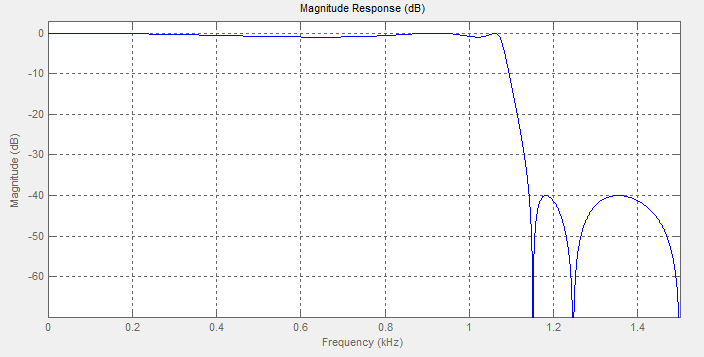
\includegraphics[width=12cm]{pictures/Filtro1/Magnitude.png}
 \caption{Resposta em frequência em magnitude do filtro I}
 \label{fig:magnitude1}
\end{figure}

\begin{figure}[ht]
 \centering
 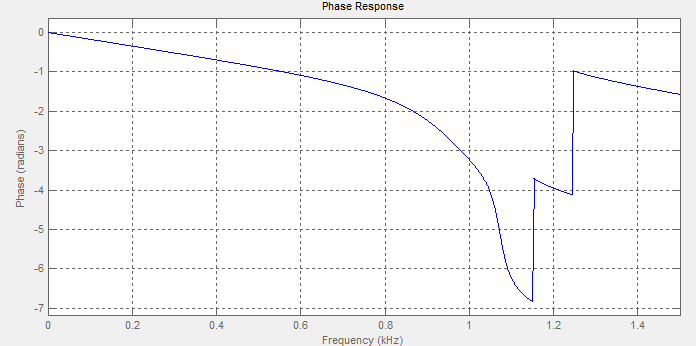
\includegraphics[width=12cm]{pictures/Filtro1/Fase.png}
 \caption{Resposta em frequência em fase do filtro I}
 \label{fig:fase1}
\end{figure}

O gráfico da resposta ao impulso e o diagrama de polos e zeros estão nas figuras \ref{fig:resimp1} e \ref{fig:diapolozero1}, respectivamente.

\begin{figure}[ht]
 \centering
 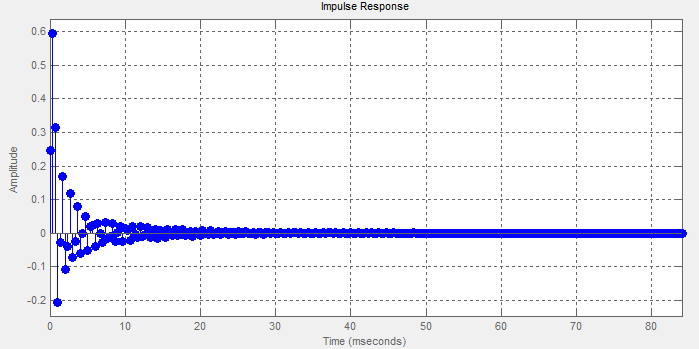
\includegraphics[width=12cm]{pictures/Filtro1/RespImpulso.png}
 \caption{Resposta ao impulso do filtro I}
 \label{fig:resimp1}
\end{figure}

\begin{figure}[ht]
 \centering
 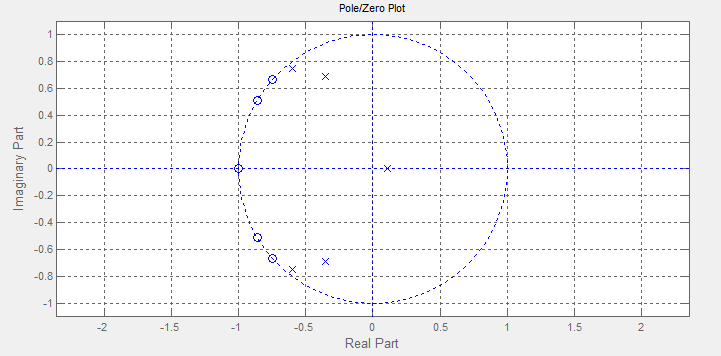
\includegraphics[width=10cm]{pictures/Filtro1/Polos&Zeros.png}
 \caption{Diagrama de polos e zeros do filtro I}
 \label{fig:diapolozero1}
\end{figure}

\begin{figure}[ht]
 \centering
 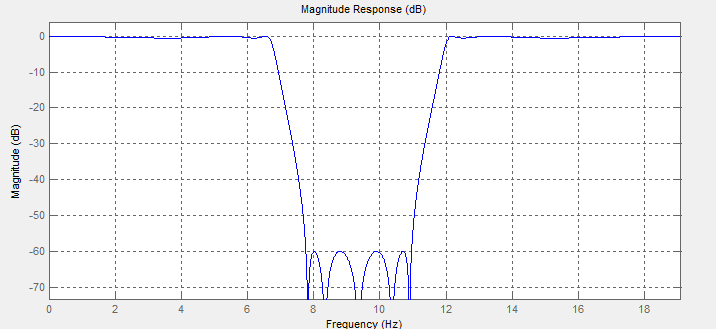
\includegraphics[width=12cm]{pictures/Filtro2/Magnitude.png}
 \caption{Resposta em frequência em magnitude do filtro II}
 \label{fig:magnitude2}
\end{figure}

\begin{figure}[ht]
 \centering
 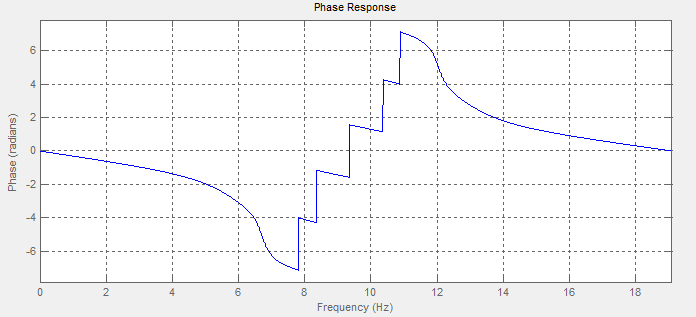
\includegraphics[width=12cm]{pictures/Filtro2/Fase.png}
 \caption{Resposta em frequência em fase do filtro II}
 \label{fig:fase2}
\end{figure}

O gráfico da resposta ao impulso e o diagrama de polos e zeros estão nas figuras \ref{fig:resimp2} e \ref{fig:diapolozero2}, respectivamente.

\begin{figure}[ht]
 \centering
 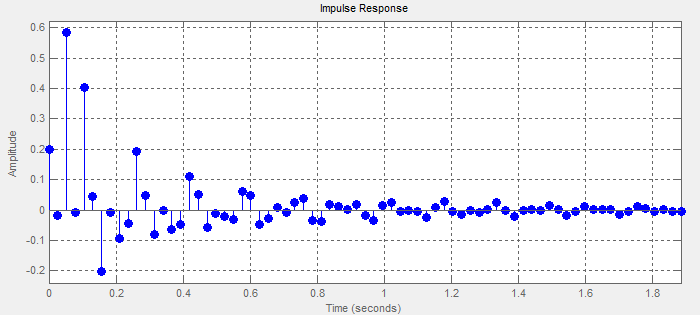
\includegraphics[width=12cm]{pictures/Filtro2/RespImpulso.png}
 \caption{Resposta ao impulso do filtro II}
 \label{fig:resimp2}
\end{figure}

\begin{figure}[ht]
 \centering
 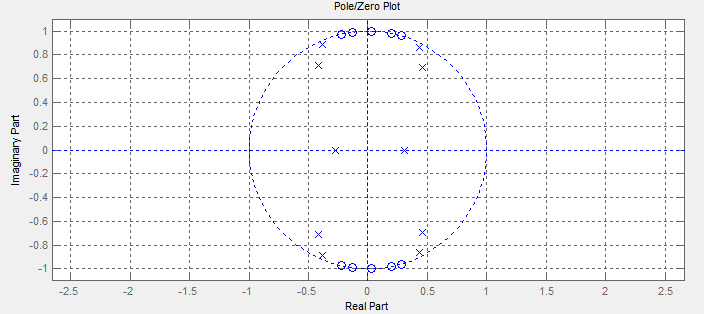
\includegraphics[width=12cm]{pictures/Filtro2/Polos&Zeros.png}
 \caption{Diagrama de polos e zeros do filtro II}
 \label{fig:diapolozero2}
\end{figure}



\end{document}
